As mentioned earlier (see section \ref{sec:intro}) one of the challenges for the agents is to decide when to perform certain actions such as avoidance for the intruder and coverage,pursuit and exploration for the guards. In order to achieve the decision-making process, three different states are created for both guards and the intruder. The three states for the guards are Exploration, Patrolling and Catching, and the three states for the intruders are Exploration, Direct-to-Target and Avoidance. Figure~\ref{fig:guardState} and Figure~\ref{fig:thiefState} show the state machines of guards and the intruder.
    Both guards and intruder start off in exploration state where guards try to learn the entire map and intruder tries to find the location of the target. Once the exploration is done for a guard, it switches to patrolling state where it tries to corporate with other guards in order to cover most of the map under their vision. The guards switch to the catching state once an intruder is identified while being in either Exploration or Patrolling states. On the other hand, once an an intruder realises the position of the target, it tries to find the shortest path towards the target, this is referred as the Direct-to-Target state in Figure~\ref{fig:thiefState}. However, since the intruder needs to avoid the guards, the avoidance state is added to the state machine. Starting either in exploration or Direct-to-Target state, the avoidance state triggers once the intruder notices guard(s) around.
\begin{figure}[H]
\centering

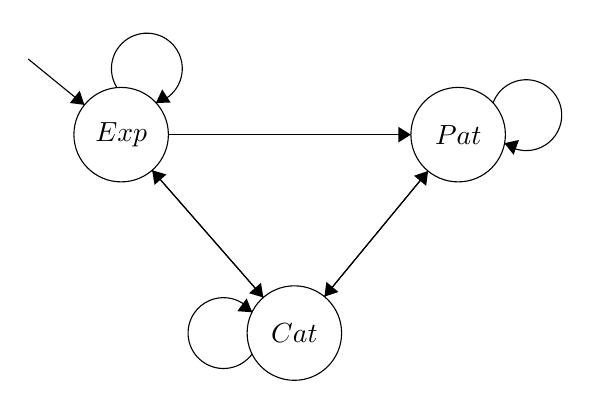
\begin{tikzpicture}[scale=0.2]
\tikzstyle{every node}+=[inner sep=0pt]
\draw [black] (12.3,-7) circle (3);
\draw (12.3,-7) node {$Exp$};
\draw [black] (33.7,-7) circle (3);
\draw (33.7,-7) node {$Pat$};
\draw [black] (23.3,-19.6) circle (3);
\draw (23.3,-19.6) node {$Cat$};
\draw [black] (14.27,-9.26) -- (21.33,-17.34);
\fill [black] (21.33,-17.34) -- (21.18,-16.41) -- (20.42,-17.07);
\draw [black] (21.33,-17.34) -- (14.27,-9.26);
\fill [black] (14.27,-9.26) -- (14.42,-10.19) -- (15.18,-9.53);
\draw [black] (15.3,-7) -- (30.7,-7);
\fill [black] (30.7,-7) -- (29.9,-6.5) -- (29.9,-7.5);
\draw [black] (12.041,-4.023) arc (212.71151:-75.28849:2.25);
\fill [black] (14.51,-4.98) -- (15.45,-4.97) -- (14.91,-4.13);
\draw [black] (35.913,-4.992) arc (159.9454:-128.0546:2.25);
\fill [black] (36.64,-7.54) -- (37.22,-8.28) -- (37.56,-7.34);
\draw [black] (31.79,-9.31) -- (25.21,-17.29);
\fill [black] (25.21,-17.29) -- (26.1,-16.99) -- (25.33,-16.35);
\draw [black] (20.62,-20.923) arc (-36:-324:2.25);
\fill [black] (20.62,-18.28) -- (20.27,-17.4) -- (19.68,-18.21);
\draw [black] (25.21,-17.29) -- (31.79,-9.31);
\fill [black] (31.79,-9.31) -- (30.9,-9.61) -- (31.67,-10.25);
\draw [black] (6.4,-2.2) -- (9.97,-5.11);
\fill [black] (9.97,-5.11) -- (9.67,-4.21) -- (9.04,-4.99);
\end{tikzpicture}

\caption{State machine of the guard. Where $Exp$, $Pat$ and $Cat$ stand for Exploration,Patrolling and Catching states respectively.}
\label{fig:guardState}
\end{figure}

\begin{figure}[H]
\centering
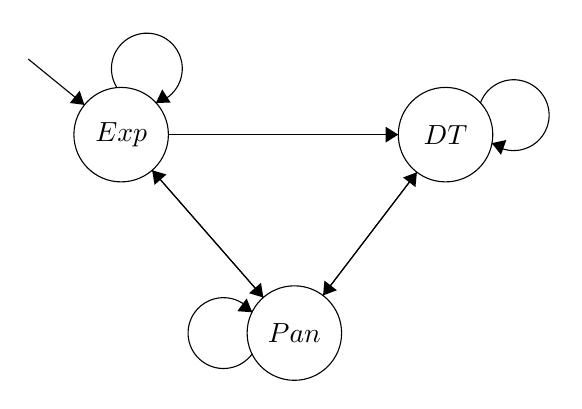
\begin{tikzpicture}[scale=0.2]
\tikzstyle{every node}+=[inner sep=0pt]
\draw [black] (12.3,-7) circle (3);
\draw (12.3,-7) node {$Exp$};
\draw [black] (32.9,-7) circle (3);
\draw (32.9,-7) node {$DT$};
\draw [black] (23.3,-19.6) circle (3);
\draw (23.3,-19.6) node {$Pan$};
\draw [black] (14.27,-9.26) -- (21.33,-17.34);
\fill [black] (21.33,-17.34) -- (21.18,-16.41) -- (20.42,-17.07);
\draw [black] (21.33,-17.34) -- (14.27,-9.26);
\fill [black] (14.27,-9.26) -- (14.42,-10.19) -- (15.18,-9.53);
\draw [black] (15.3,-7) -- (29.9,-7);
\fill [black] (29.9,-7) -- (29.1,-6.5) -- (29.1,-7.5);
\draw [black] (12.041,-4.023) arc (212.71151:-75.28849:2.25);
\fill [black] (14.51,-4.98) -- (15.45,-4.97) -- (14.91,-4.13);
\draw [black] (35.113,-4.992) arc (159.9454:-128.0546:2.25);
\fill [black] (35.84,-7.54) -- (36.42,-8.28) -- (36.76,-7.34);
\draw [black] (31.08,-9.39) -- (25.12,-17.21);
\fill [black] (25.12,-17.21) -- (26,-16.88) -- (25.21,-16.27);
\draw [black] (20.62,-20.923) arc (-36:-324:2.25);
\fill [black] (20.62,-18.28) -- (20.27,-17.4) -- (19.68,-18.21);
\draw [black] (25.12,-17.21) -- (31.08,-9.39);
\fill [black] (31.08,-9.39) -- (30.2,-9.72) -- (30.99,-10.33);
\draw [black] (6.4,-2.2) -- (9.97,-5.11);
\fill [black] (9.97,-5.11) -- (9.67,-4.21) -- (9.04,-4.99);
\end{tikzpicture}
\caption{State machine of the intruder. Where $Exp$, $DT$ and $Avoid$ stand for Exploration, Direct-to-Target and Avoidance states respectively}
\label{fig:thiefState}
\end{figure}

